\documentclass[]{article}
\usepackage{graphicx}
\usepackage[spanish]{babel}
\usepackage[a4paper, top=2.5cm, bottom=2.5cm, left=3cm, right=3cm]{geometry}
\usepackage[hidelinks]{hyperref}
\usepackage[T1]{fontenc}
\usepackage{listings}
\usepackage{xcolor}
\usepackage{float}

\definecolor{miverde}{rgb}{0,0.6,0}
\definecolor{aqua}{rgb}{0.0, 0.5, 0.8}
\definecolor{miotrootroverde}{rgb}{0.11, 0.40, 0.11}
\lstdefinelanguage{JavaScript}{
  keywords={typeof, new, true, false, catch, function, return, null, catch, switch, var, if, in, while, do, else, case, break, $sum, $out, $size, $filter, $group, $addFields, $substract, $multiply, $divide, $round, $map, $reduce, $replaceRoot, $mergeObjects, $unwind, $dateFromString, $floor, $project, $jsonSchema, $lookup},
  keywordstyle=\color{blue}\bfseries,
  ndkeywords={class, export, boolean, throw, implements, import, this, validator, db, createCollection, bsonType, description, title, required, properties},
  ndkeywordstyle=\color{miotrootroverde}\bfseries,
  identifierstyle=\color{aqua},
  sensitive=false,
  comment=[l]{//},
  morecomment=[s]{/*}{*/},
  commentstyle=\color{red}\ttfamily,
  stringstyle=\color{miverde}\ttfamily,
  morestring=[b]',
  morestring=[b]"
}
% style for listings (código)
\lstdefinestyle{python}{
    language=Python,
    backgroundcolor=\color{gray!2},     % Color de fondo
    basicstyle=\ttfamily,               % Tipo y tamaño de fuente
    keywordstyle=\color{blue}\bfseries, % Color para palabras clave
    stringstyle=\color{miverde},        % Color para cadenas
    commentstyle=\color{red},           % Color para comentarios
    showspaces=false,                   % No mostrar espacios
    showstringspaces=false,             % No mostrar espacios en las cadenas
    frame=single,                       % Poner un marco alrededor del código
    breaklines=true,                    % Romper las líneas largas
    captionpos=b,                       % Posición del caption
    tabsize=4,                          % Tamaño de las tabulaciones
    escapeinside={\%*}{*)},             % Para incluir código LaTeX en los listings
    morekeywords={self}                 % Palabras clave adicionales
}

\lstdefinestyle{bash}{
    language=shell,
    backgroundcolor=\color{gray!2},     % Color de fondo
    basicstyle=\ttfamily,               % Tipo y tamaño de fuente
    keywordstyle=\color{blue}\bfseries, % Color para palabras clave
    stringstyle=\color{miverde},        % Color para cadenas
    commentstyle=\color{red},           % Color para comentarios
    showspaces=false,                   % No mostrar espacios
    showstringspaces=false,             % No mostrar espacios en las cadenas
    frame=single,                       % Poner un marco alrededor del código
    breaklines=true,                    % Romper las líneas largas
    captionpos=b,                       % Posición del caption
    tabsize=4,                          % Tamaño de las tabulaciones
    escapeinside={\%*}{*)},             % Para incluir código LaTeX en los listings
    morekeywords={self}                 % Palabras clave adicionales
}

\lstset{basicstyle=\ttfamily}
\lstset{
    inputencoding=utf8,
    extendedchars=true,      % Permitir caracteres extendidos (acentos)
    literate=%
        {á}{{\'a}}1 {Á}{{\'A}}1
        {é}{{\'e}}1 {É}{{\'E}}1
        {í}{{\'i}}1 {Í}{{\'I}}1
        {ó}{{\'o}}1 {Ó}{{\'O}}1
        {ú}{{\'u}}1 {Ú}{{\'U}}1
}


%title
\title{Práctica 2} 

\author{Adrián Ferández Galán, César López Mantecón y Manuel Gómez-Plana Rodríguez}

\begin{document}

\begin{titlepage}
    \centering
   
\includegraphics[width=0.9\textwidth]{uc3m.jpg} 
    {\Huge Universidad Carlos III\\
    
     \Large Arquitectura de Datos\\
     \vspace{0.5cm}
     Curso 2024-25}
    \vspace{2cm}

    {\Huge \textbf{Práctica 1.2} \par}
    \vspace{0.5cm}
    {\Large Diseño de los clusters \par}
    \vspace{8cm}

   \textbf{Ingeniería Informática, Cuarto curso}\\
    \vspace{0.2cm} 
    Adrián Fernández Galán       (NIA: 100472182, e-mail: 100472182@alumnos.uc3m.es)\\
    César López Mantecón         (NIA: 100472092, e-mail: 100472092@alumnos.uc3m.es)\\
    Manuel Gómez-Plana Rodríguez (NIA: 100472310, e-mail: 100472310@alumnos.uc3m.es)
    \vspace{0.5cm}

   
    \textbf{Prof.} Lourdes Moreno López\\
    
    \textbf{Grupo: } 81   
    
\end{titlepage}
\newpage

\renewcommand{\contentsname}{\centering Índice}
\tableofcontents

\newpage
\section{Introducción}
\label{sec:introduccion}
En este documento se discutirá del diseño de los clusters de la base de datos sobre las areas recreativas de Madrid. Para este diseño se hablarán de las diferentes posibilidades que se pueden conseguir a través de la \textbf{fragmentación} y de la \textbf{replicación}, además de analizar sus consecuencias tanto en el contexto de nuestra base de datos como en contextos parecidos.
\newpage
\lstset{style=python}
\section{Fragmentación}
\label{sec:fragmentacion}
En este apartado se analizarán las diferentes estrategias con las que se podrán abordar para cada una de las colecciones de los distintos agregados.

\subsection{Clave de Fragmentación}
\label{subsec:fragmmentacion}

\subsubsection{Agregado Area\_Recreativa\_Clima}
\label{subsubsec:fragmentacion_area}
Dada las características del agregado de \texttt{Area\_Recreativa\_Clima} proponemos 5 posibles claves de fragmentación que nos permitan repartir de la carga de los casos de uso: \textit{\_id}, \textit{Cod\_Barrio}, \textit{Cod\_Distrito}, \textit{Cod\_Postal} y \textit{Fecha\_Instalacion}. A continuación se analizarán las propuestas de clave de fragmentación.

\begin{itemize}
    \item \textbf{\textit{\_id}}
    
    Esta clave de fragmentación correponde con el tipo de \textbf{clave aleatoria}, debido a que sus valores no siguen ningún tipo de patrón, ni su valor está relacionado con otra columna. Esta condición permite que los datos se distribuyan de manera uniforme, sin embargo, esto también puede causar que los datos ubicados en cada \textit{shard} no tengan una relación entre ellos, lo que aumentaría la carga de lecturas de datos por intervalos.

    \item \textbf{\textit{Cod\_Barrio}} y \textbf{\textit{Cod\_Distrito}}
    
    Analizamos estas claves por igual ya que son tienen las mismas características y por ello los mismos resultados. Estas claves de fragmentacion corresponden con el tipo de \textbf{clave basada en la localización}, lo que distribuirá los datos con las mismas ubicaciones en los mismos shards, sin embargo es necesario conocer cómo se distribuyen los datos, para asegurarse que no existen desbalanceos. A continuación podemos ver la distribución de los datos para estas claves.

    \begin{figure}[H]
        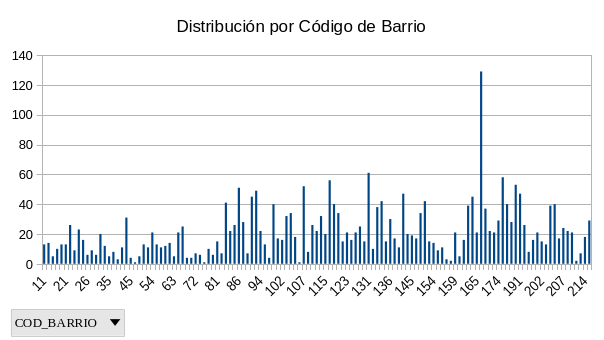
\includegraphics[width=0.45\linewidth]{Distribucion_Cod_Barrio.png}
        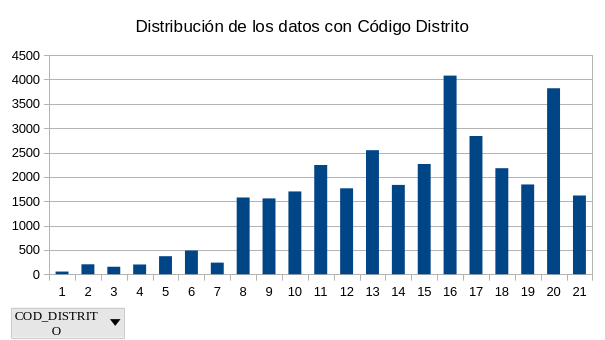
\includegraphics[width=0.45\linewidth]{Distribucion_Cod_Distrito.png}
        \caption{Distribución de los datos para ambas claves}
    \end{figure}

    \item \textbf{\textit{DESC\_CLASIFICACION}}
    
    Al igual que las anteriores, esta columna funciona como \textbf{clave basada en localización}, por lo que tiene las mismas ventajas y desventajas que \textit{Cod\_Barrio} y \textit{Cod\_Distrito}. A continuación mostramos la distribución de los datos con esta clave.

    \begin{figure}[H]
        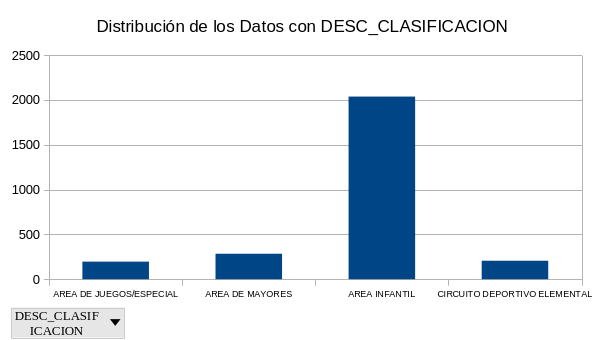
\includegraphics[width=0.90\linewidth]{Distribucion_DESC_CLASIFICACION.png}
        \caption{Distribución de los datos para la clave \textit{DESC\_CLASIFICACION}}
    \end{figure}

    \item \textbf{\textit{Cod\_Postal}}
    
    Al igual que para las anteriores claves, esta clave es del tipo \textbf{clave basada en la localización}, por lo que aquellas áreas con el mismo código postal se ubicarán en los mismos shards, lo que reducirá la carga de las lecturas en intervalos o en grupos. A diferencia de \textit{Cod\_Barrio} y \textit{Cod\_Distrito}, las áreas de un mismo shard siempre tendrán el mismo clima, dada la naturaleza de la relación entre la tabla \textit{area} y la tabla \textit{meteo}. A continuación podemos ver la distribución de los datos para esta clave.
    \begin{figure}[H]
        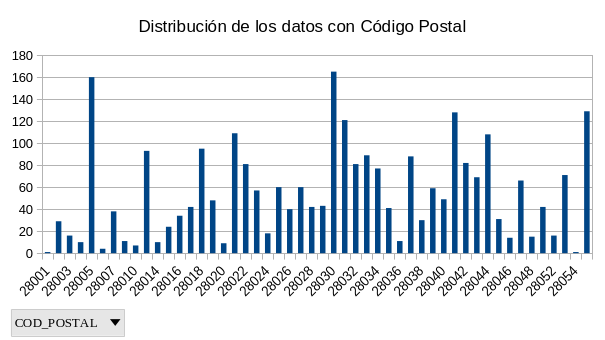
\includegraphics[width=0.90\linewidth]{Distribucion_Cod_Postal.png}
        \caption{Distribución de los datos para la clave \textit{Cod\_Postal}}
    \end{figure}

    \item \textbf{\textit{Fecha\_Instalación}}
    
    Esta clave de fragmentacion corresponde con el tipo de \textbf{claves ascendientes}, dado que es un valor que aumenta de forma secuencial y nuevas instancias tomarán siempre valores más grandes que los ya existentes. Esta característica hará que aquellas fechas más cercanas se encuentren en el mismo shard, lo que facilita la lectura por intervalos de fecha. Sin embargo, perjudicará a las escrituras, ya que todas las nuevas instanias irán a parar al último \textit{shard}, lo que aumentará la carga de este.

    
    
\end{itemize}

\subsubsection{Agregado Juegos}
\label{subsubsec:fragmentacion_juegos}

Como en el agregado de \textit{Juegos} tenemos las mismas columnas que en el agregado de \textit{Areas} podemos proponer las mismas claves de partición en para el anterior agregado. En este caso desecharemos las claves de partición para \textit{\_id} y \textit{Fecha\_Instalación}, dado que consideramos que las claves aleatorias y ascendentes no se ajustan a las características de nuestros casos de uso. A continuación analizaremos las columnas \textit{Cod\_Barrio}, \textit{Cod\_Distrito} y \textit{Cod\_Postal}.

\begin{itemize}
    \item \textbf{\textit{Cod\_Barrio}} y \textbf{\textit{Cod\_Distrito}}
    
    Como hemos mencionado en la anterior sección estas claves corresponden con el tipo de \textbf{clave basada en la localización}, lo que permite tener en un mismo fragmento aquellos datos que se encuentren en ubicaciones cercanas, reduciendo la carga de las lecturas en grupos. Sin embargo, puede ocurrir que existan fragmentos con mucha más carga que otros dada la distribución de los datos. Para ello visualizaremos las distribuiciones de los datos para ambas claves de partición.

    \begin{figure}[H]
        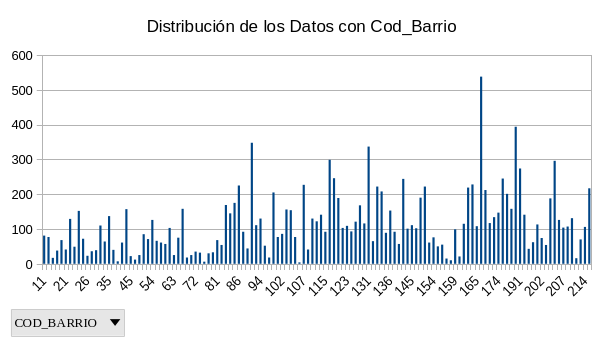
\includegraphics[width=0.45\linewidth]{Distribucion_Juegos_Cod_Barrio.png}
        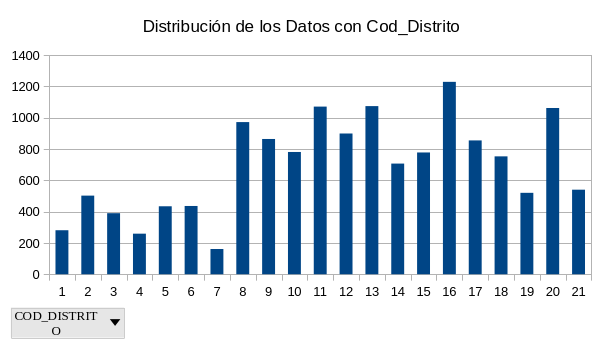
\includegraphics[width=0.45\linewidth]{Distribucion_Juegos_Cod_Distrito.png}
        \caption{Distribución de los datos para ambas claves}
    \end{figure}

    \item \textbf{\textit{DESC\_CLASIFICACION}}
    
    Al igual que las anteriores, esta columna funciona como \textbf{clave basada en localización}, por lo que tiene las mismas ventajas y desventajas que \textit{Cod\_Barrio} y \textit{Cod\_Distrito}. A continuación mostramos la distribución de los datos con esta clave.

    \begin{figure}[H]
        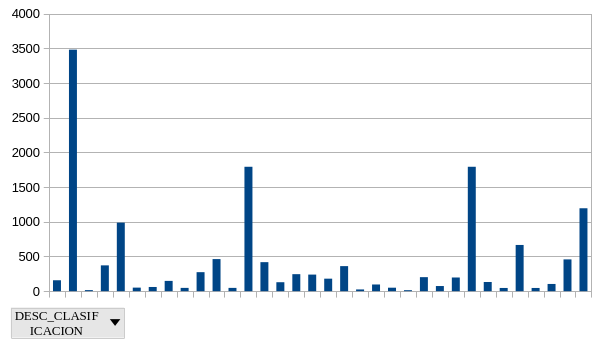
\includegraphics[width=0.90\linewidth]{Distribucion_Juegos_DESC_CLASIFICACION.png}
        \caption{Distribución de los datos para la clave \textit{DESC\_CLASIFICACION}}
    \end{figure}

    \item \textbf{\textit{Cod\_Postal}}
    
    Al igual que para el anterior agregado \textit{Cod\_Postal} funciona como \textbf{clave basada en la localización}, sin embargo en este caso existen \textit{missing values}, por lo que no nos sirve como clave de partición debido a que no todos los registros podrán identificarse en un \textit{shard}.
\end{itemize}

\subsubsection{Agregado Incidencias de Usuario}
\label{subsubsec:fragmentacion_incidencias}

Para este agregado las propuestas para la clave de partición son las siguientes:

\begin{itemize}
    \item \textbf{\textit{\_id}}
    
    La clave \textit{\_id} es del tipo \textbf{clave ascendiente}, como para el resto de casos no es una buena clave de fragmentacion dadas las características de los casos de uso.

    \item \textbf{\textit{TIPO\_INCIDENCIA}}
    
    La clave \textit{TIPO\_INCIDENCIA} es del tipo \textbf{clave basada en la localización}, y para evaluar la calidad de esta clave visualizaremos la distribución de los datos.

    \begin{figure}[H]
        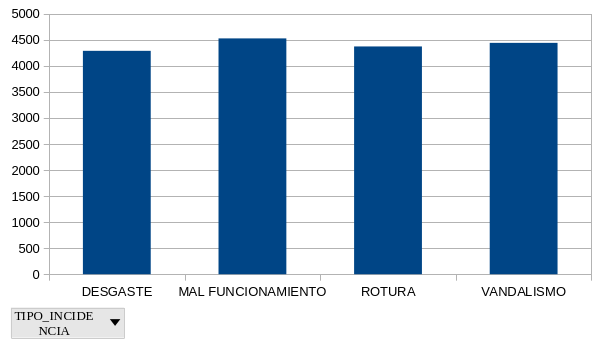
\includegraphics[width=0.90\linewidth]{Distribucion_Incidencias_TIPO_INCIDENCIA.png}
        \caption{Distribución de los datos para la clave \textit{TIPO\_INCIDENCIA}}
    \end{figure}

    \item \textbf{\textit{FECHA\_REPORTE}}
    
    La clave \textit{FECHA\_REPORTE} es del tipo \textbf{clave ascendente}, como para el resto de casos no es una buena clave de fragmentacion dadas las características de los casos de uso.

\end{itemize}










\end{document}
